\documentclass[border=2pt]{standalone}
\usepackage{tikz}
\usetikzlibrary{shapes.misc,shapes.multipart}
\begin{document}
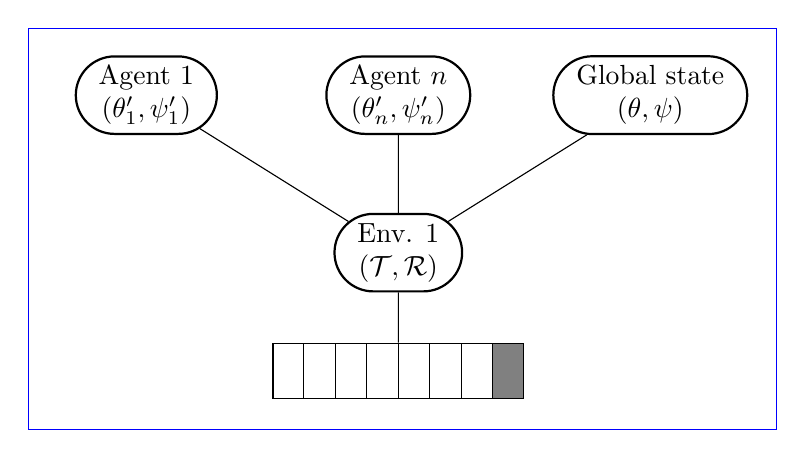
\begin{tikzpicture}
  \draw[blue] (-1.5,-4.25) rectangle (8,.85);
  \node[rounded rectangle,draw,thick,align=center] (A1) at (0,0)
    {Agent 1\\$(\theta_1', \psi_1')$};
  \node[rounded rectangle,draw,thick,align=center] (AN) at (3.2,0)
    {Agent $n$\\$(\theta_n', \psi_n')$};
  \node[rounded rectangle,draw,thick,align=center] (G) at (6.4,0)
    {Global state\\$(\theta, \psi)$};
  \node[rounded rectangle,draw,thick,align=center] (E1) at (3.2,-2)
    {Env. 1\\$(\mathcal{T}, \mathcal{R})$};
  \node[rectangle split,minimum height=.7cm,rectangle split horizontal,
    rectangle split parts=8,draw,
    rectangle split part fill={white,white,white,white,white,white,white,gray}]
    (q1) at (3.2,-3.5) {};
  \draw (A1) -- (E1) (AN) -- (E1) (G) -- (E1) (E1) -- (q1);
\end{tikzpicture}
\end{document}
